\documentclass{llncs}
\usepackage{times}
\usepackage[T1]{fontenc}

% Comentar para not MAC Users
%\usepackage[applemac]{inputenc}

\usepackage{a4}
%\usepackage[margin=3cm,nohead]{geometry}
\usepackage{epstopdf}
\usepackage{indentfirst}
\usepackage{graphicx}
\graphicspath{{Capturas-Ecra/}}
\usepackage{float}
\usepackage{fancyvrb}
\usepackage{amsmath}
\usepackage{array}
%\renewcommand{\baselinestretch}{1.5}


\begin{document}
\mainmatter
\title{TP3 - Serviço de Resolução de Nomes (DNS)}

\titlerunning{TP3 - Serviço de Resolução de Nomes (DNS)}

\author{Diogo Braga \and João Silva}

\authorrunning{Diogo Braga \and João Silva}

\institute{
University of Minho, Department of  Informatics, 4710-057 Braga, Portugal\\
e-mail: \{a82547,a82005\}@alunos.uminho.pt\\
PL2, Grupo 6
}

\date{}
\bibliographystyle{splncs}

\maketitle

\section{Questões e Respostas}

\subsection{\textbf{Qual o conteúdo do ficheiro /etc/resolv.conf e para que serve essa informação?}}
\textbf{R:} Este ficheiro contém o nome do domínio de procura e os servidores que respondem a este nome. O domínio corresponde ao nome do domínio local. O nameserver é responsável pelo endereço de internet pela qual o \textit{resolver} irá interrogar.


\subsection{\textbf{Os servidores www.google.pt. e www.google.com. têm endereços IPv6? Se sim, quais?}}
\textbf{R:} Como mostra a figura \ref{fig:1b1}, utilizando a ferramenta \textbf{dig} para interrogar sobre o servidor \textbf{www.google.pt.}, e reparando no resource record definido como \textbf{AAAA}, é possível verificar que este possui endereços IPv6 nos servidores ns2,ns1,ns3 e ns4.

\begin{figure}[H]
\begin{center}
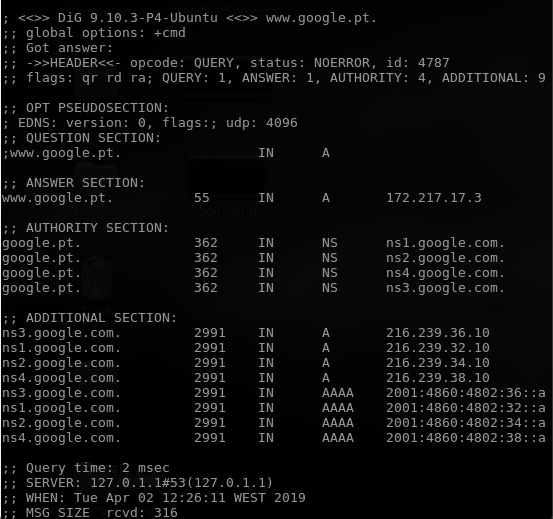
\includegraphics[scale=0.5]{2_1.png}
\end{center}
\caption{\label{fig:1b1}Dig \textbf{www.google.pt.}}
\end{figure}


\newpage

Fazendo o mesmo para o servidor \textbf{www.google.com.}, é possível verificar que também existem endereços IPv6. Estes endereços são os mesmos que os apresentados para o www.google.pt..

\begin{figure}[H]
\begin{center}
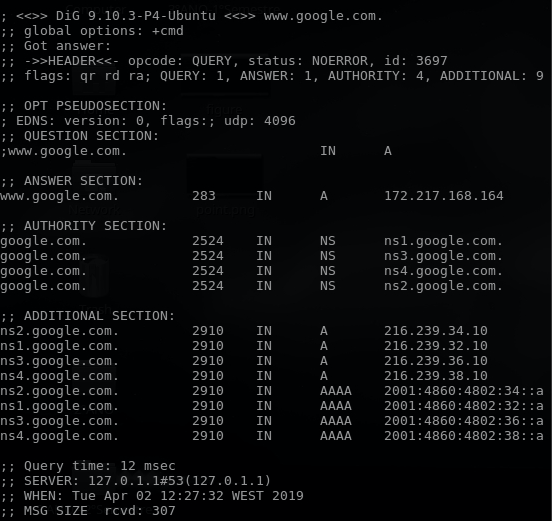
\includegraphics[scale=0.5]{2_2.png}
\end{center}
\caption{\label{fig:1b1}Dig \textbf{www.google.com.}}
\end{figure}


\subsection{\textbf{Quais os servidores de nomes definidos para os domínios: "ccg.pt.", "pt." e "."?}}
\textbf{R:} Tal como pode ser verificado na figura \ref{fig:31}, no domínio \textbf{ccg.pt.}, os nomes definidos para os servidores são \textbf{ns1.ccg.pt.} e \textbf{ns3.ccg.pt.}. Tal é verificável através do resource record definido \textbf{NS}.

\begin{figure}[H]
\begin{center}
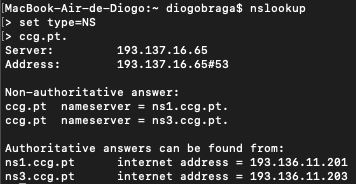
\includegraphics[scale=0.6]{3_1.png}
\end{center}
\caption{\label{fig:31}Nslookup NS \textbf{ccg.pt.}}
\end{figure}


\newpage

Quanto ao domínio \textbf{pt.}, os nomes definidos para os servidores estão definidos dentro da secção vermelha representada na figura \ref{fig:32}.

\begin{figure}[H]
\begin{center}
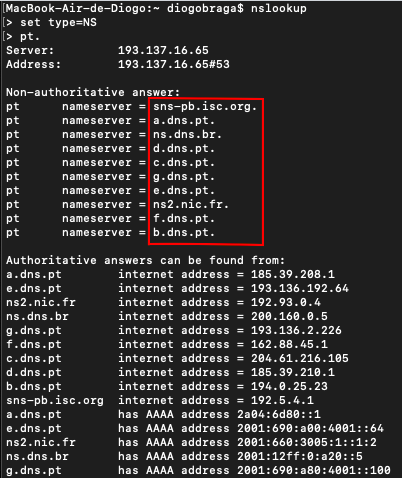
\includegraphics[scale=0.6]{3_2.png}
\end{center}
\caption{\label{fig:32}Nslookup NS \textbf{pt.}}
\end{figure}

\newpage

Na figura \ref{fig:33} é possível concluir quais são os nomes definidos para os servidores do domínio \textbf{.}. Tais estão representados na secção vermelha.

\begin{figure}[H]
\begin{center}
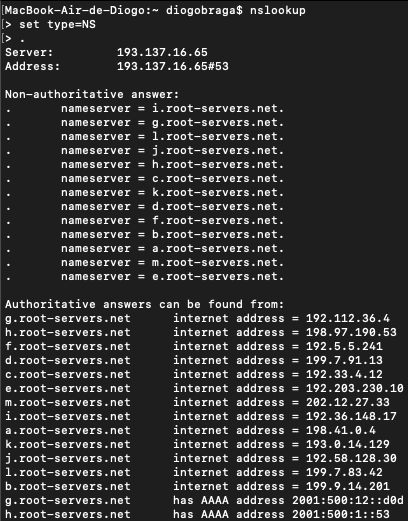
\includegraphics[scale=0.6]{3_3.png}
\end{center}
\caption{\label{fig:33}Nslookup NS \textbf{.}}
\end{figure}


\newpage

\subsection{\textbf{Existe o domínio eureka.software.? Será que eureka.software. é um host?}}
\textbf{R:} Como é possível verificar na figura \ref{fig:4}, as linhas verdes demonstram que existe o domínio \textbf{eureka.software.}, pois este possui resource records definidos como NS. Nesta secção estão, então, os nomes dos hosts do servidor DNS autoritativo do domínio.

Na mesma figura, a linha vermelha mostra que o \textbf{eureka.software.} também é um host, pois este possui um resource record definido como A, que significa que eureka.software é um nome de um host, e que 34.214.90.141 é o endereço IP associado.

\begin{figure}[H]
\begin{center}
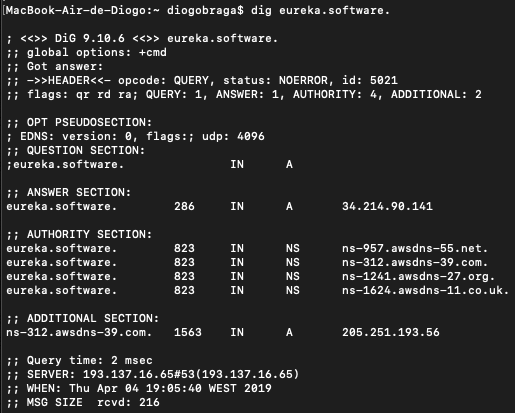
\includegraphics[scale=0.6]{4.png}
\end{center}
\caption{\label{fig:4}Dig \textbf{eureka.software.}}
\end{figure}


\subsection{\textbf{Qual é o servidor DNS primário definido para o domínio ami.pt.? Este servidor primário (master) aceita queries recursivas? Porquê?}}
\textbf{R:} O servidor primário do domínio ami.pt. pode ser revelado executando a ferramenta nslookup e estabelecendo como filtro o tipo \textbf{SOA}(Start Of Authority), que define o início de uma zona e todos os seus parâmetros.

Pela figura \ref{fig:5}, é possível verificar o campo \textbf{origin}, que tem como correspondência o domínio \textbf{ns1.dot2web.com}, sendo este o definido como servidor DNS primário.

Concluimos que este servidor aceita queries recursivas, pois efetuando o \textbf{dig ns1.dot2web.com}, é possível verificar a presença das flags \textbf{RD Recursion Desired} e \textbf{RA Recursion Available} na figura \ref{fig:521}, sublinhado a vermelho.

\begin{figure}[H]
\begin{center}
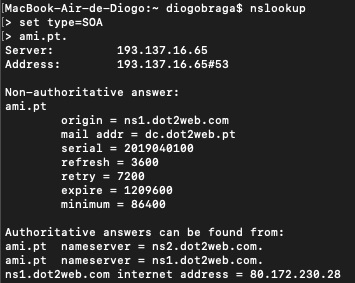
\includegraphics[scale=0.6]{5.png}
\end{center}
\caption{\label{fig:5}Nslookup SOA \textbf{ami.pt.}}
\end{figure}

\begin{figure}[H]
\begin{center}
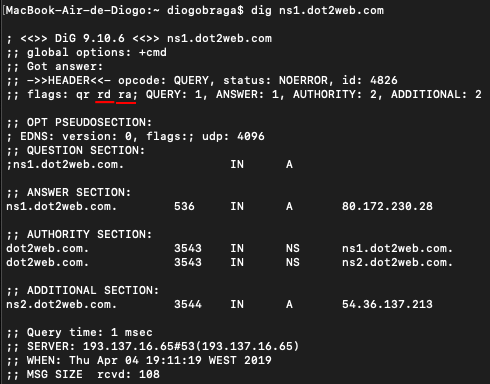
\includegraphics[scale=0.6]{5_1.png}
\end{center}
\caption{\label{fig:521}Dig \textbf{ns1.dot2web.com}}
\end{figure}


\newpage

\subsection{\textbf{Obtenha uma resposta "autoritativa" para a questão anterior.}}
\textbf{R:} Uma resposta autoritativa, como se pode verificar na figura \ref{fig:522}, pode ser o nameserver \textbf{ns2.dot2web.com.}.

\begin{figure}[H]
\begin{center}
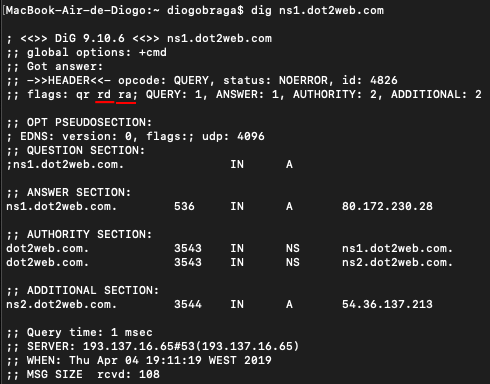
\includegraphics[scale=0.6]{5_2.png}
\end{center}
\caption{\label{fig:522}Nslookup SOA \textbf{ami.pt.}}
\end{figure}

\subsection{\textbf{Onde são entregues as mensagens dirigidas a marcelo@presidencia.pt ? E a guterres@onu.org?}}
\textbf{R:} Como é possível verificar na figura \ref{fig:71}, as mensagens dirigidas a marcelo@presidencia.pt serão entregues, em primeiro caso, a \textbf{mail2.presidencia.pt} e, caso este se encontre indisponível, serão entregues a \textbf{mail.presidencia.pt}. Para tal conclusão definimos o tipo \textbf{MX}, que filtra os nomes dos servidores de e-mail associados ao nome do domínio.

Importante referir que o servidor \textbf{mail2} tem prioridade em relação ao servidor \textbf{mail}, pois o primeiro aqui na frase referenciado tem prioridade 10 enquanto o segundo tem prioridade 50. Tal acontece porque quanto menor for o número, maior é a prioridade.

\begin{figure}[H]
\begin{center}
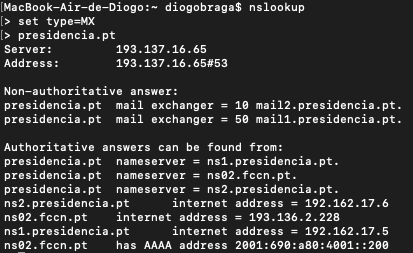
\includegraphics[scale=0.6]{7_1.png}
\end{center}
\caption{\label{fig:71}Nslookup MX \textbf{presidencia.pt}}
\end{figure}

Por outro lado, e definindo de igual modo o tipo \textbf{MX} como filtro, as mensagens dirigidas a guterres@onu.org serão entregues a \textbf{mail.onu.org}. Neste caso só existe uma possibilidade logo não existe opção a tomar como no caso anterior. Tal é possível verificar na figura \ref{fig:72}.

\begin{figure}[H]
\begin{center}
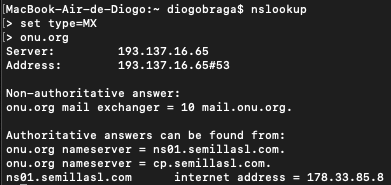
\includegraphics[scale=0.6]{7_2.png}
\end{center}
\caption{\label{fig:72}Nslookup MX \textbf{onu.org}}
\end{figure}


\subsection{\textbf{Que informação é possível obter acerca de www.whitehouse.gov? Qual é o endereço IPv4 associado?}}
\textbf{R:} Tal como mostra a figura \ref{fig:8} em baixo representada, a informação possível de obter é o endereço IP associado a um host. Tal é possível concluir devido ao resource record apresentado \textbf{(A)}. Devido a ser A ao invês de AAAA, concluimos que estamos perante IPv4. O endereço associado é, portanto, o 104.83.50.153.

\begin{figure}[H]
\begin{center}
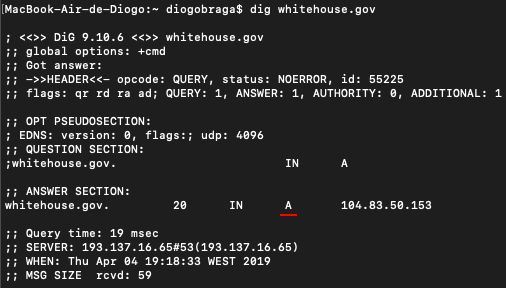
\includegraphics[scale=0.6]{8.png}
\end{center}
\caption{\label{fig:8}Dig \textbf{www.whitehouse.gov}}
\end{figure}


\subsection{\textbf{Consegue interrogar o DNS sobre o endereço IPv6 2001:690:a00:1036:1113::247 usando algum dos clientes DNS? Que informação consegue obter? Supondo que teve problemas com esse endereço, consegue obter um contacto do responsável por esse IPv6?}}
\textbf{R:} Utilizando a ferramenta nslookup e o filtro AAAA, resource record que identifica o IPv6, foi possível concluir qual o domínio a este associado.

A informação obtida foi, portanto, o nome dos servidores associados ao domínio, o endereço internet associado a cada servidor, e também como o endereço IPv6 associado a cada servidor.

Tendo problemas com esse endereço, é possível contactar o servidor web \textbf{www.fccn.pt}, que é um contacto do responsável pelo IPv6 referenciado no enunciado.


\begin{figure}[H]
\begin{center}
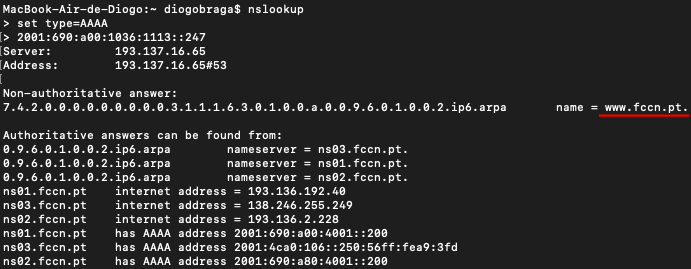
\includegraphics[scale=0.6]{9.png}
\end{center}
\caption{\label{fig:9}Nslookup AAAA \textbf{2001:690:a00:1036:1113::247}}
\end{figure}


\subsection{\textbf{Os secundários usam um mecanismo designado por "Transferência de zona" para se atualizarem automaticamente a partir do primário, usando os parâmetros definidos no Record do tipo SOA do domínio. Descreve sucintamente esse mecanismo com base num exemplo concreto (ex: di.uminho.pt ou o domínio cc.pt que vai ser criado na topologia virtual).}}
\textbf{R:} Os servidores secundários são tidos como "backups" dos servidores primários, e como tal estes necessitam de se atualizar com o conteúdo do primário periodicamente, de forma a conterem dados consistentes. Para tal, existem alguns parâmetros definidos no Record do tipo SOA do domínio.

Tendo em conta o exemplo do domínio cc.pt criado na topologia virtual, e em baixo disponibilizado em formato de imagem, é possível verificar os tais parâmetros definidos como tempo para atualização dos dados.

O campo \textbf{serial} incrementa quando os dados do servidor primário são modificados, de modo que depois o servidor secundário consiga saber quando o servidor primário foi alterado e deve ser recarregado.

O campo \textbf{refresh} demonstra o número de segundos entre as solicitações de atualização do servidor secundário. Neste caso, 604800 segundos = 7 dias.

O campo \textbf{retry} representa o número de segundos que o servidor secundário irá esperar antes de tentar novamente quando a última tentativa falhar. Neste caso, 86400 segundos = 1 dia.

O campo \textbf{expire} mostra o número de segundos que o secundário irá esperar antes de considerar os dados antigos se não conseguirem alcançar o servidor de nome principal. Neste caso, 2419200 horas = 100800 dias.

Para terminar, o campo \textbf{negative cache TTL} especifica o número de segundos que um nome de domínio é armazenado em cache localmente antes da expirar e retorna aos servidores de nomes oficiais para obter informações atualizadas. Neste caso, 86400 segundos = 1 dia.

\begin{figure}[H]
\begin{center}
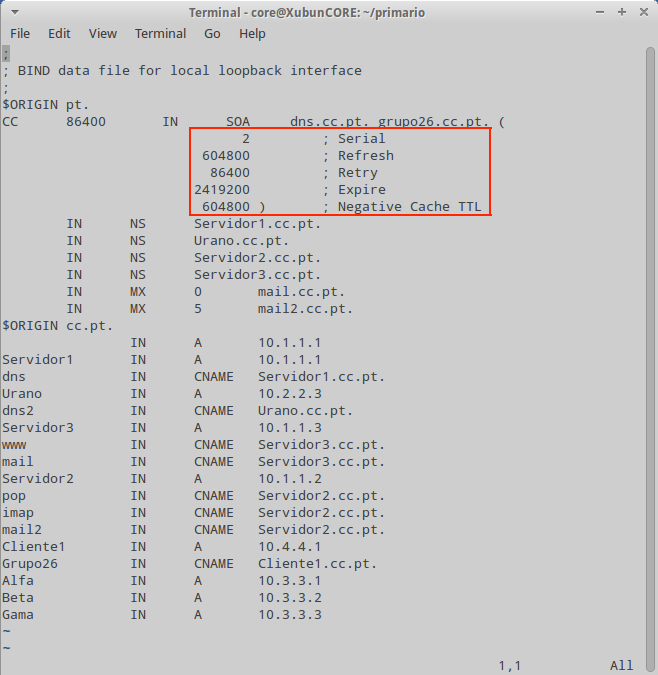
\includegraphics[scale=0.6]{10.png}
\end{center}
\caption{\label{fig:10}\textbf{db.cc.pt}}
\end{figure}


\newpage

\section{Demonstração do funcionamento do domínio de nomes CC.pt}

Nesta secção do trabalho apresentamos umas imagens que demonstram os testes realizados aos servidores primário e secundário na tentativa de ver que estes se encontravam a funcionar corretamente.

Os testes que trazemos são baseados no que o enunciado pretende. Todas as configurações que necessitamos de fazer para ambos os servidores encontram-se nas pastas \textbf{primario} e \textbf{secundario}.

\begin{figure}[H]
\begin{center}
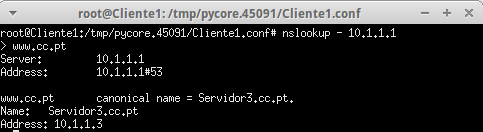
\includegraphics[scale=0.75]{teste1.png}
\end{center}
\caption{\label{fig:t1}Exemplo de Teste duma query ao servidor}
\end{figure}

\begin{figure}[H]
\begin{center}
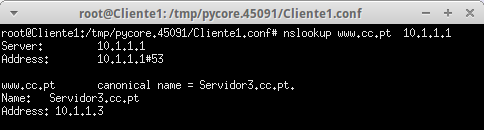
\includegraphics[scale=0.75]{teste2.png}
\end{center}
\caption{\label{fig:t2}Exemplo de Teste duma query ao servidor}
\end{figure}

\begin{figure}[H]
\begin{center}
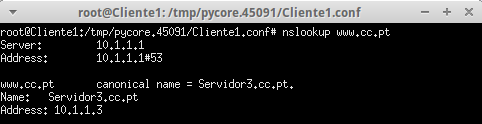
\includegraphics[scale=0.75]{teste3.png}
\end{center}
\caption{\label{fig:t3}Exemplo de Teste duma query ao servidor}
\end{figure}

\begin{figure}[H]
\begin{center}
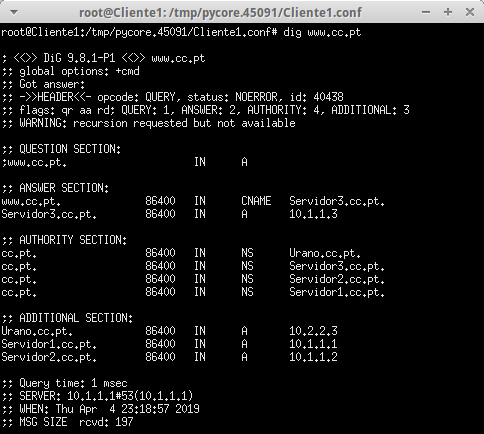
\includegraphics[scale=0.75]{teste4.png}
\end{center}
\caption{\label{fig:t4}Exemplo do comando \textbf{dig} para um servidor Web }
\end{figure}

\begin{figure}[H]
\begin{center}
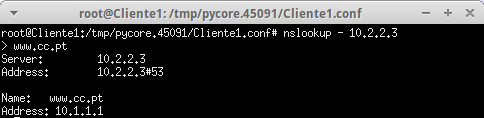
\includegraphics[scale=0.75]{teste5.png}
\end{center}
\caption{\label{fig:t5}Exemplo de Teste duma query ao servidor secundário}
\end{figure}

\begin{figure}[H]
\begin{center}
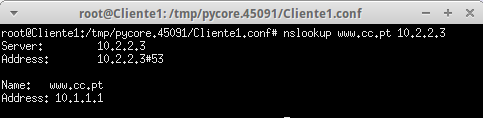
\includegraphics[scale=0.75]{teste6.png}
\end{center}
\caption{\label{fig:t6}Exemplo de Teste duma query ao servidor secundário}
\end{figure}

\begin{figure}[H]
\begin{center}
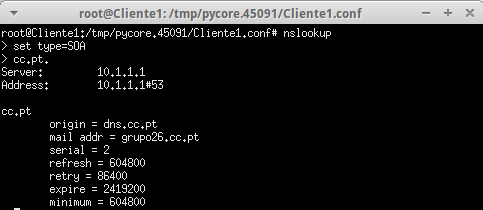
\includegraphics[scale=0.75]{teste7.png}
\end{center}
\caption{\label{fig:t7}Query do tipo SOA ao servidor.}
\end{figure}

\begin{figure}[H]
\begin{center}
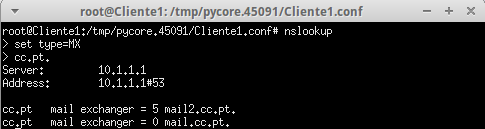
\includegraphics[scale=0.75]{teste8.png}
\end{center}
\caption{\label{fig:t8}Teste ao serviço de mail}
\end{figure}

\begin{figure}[H]
\begin{center}
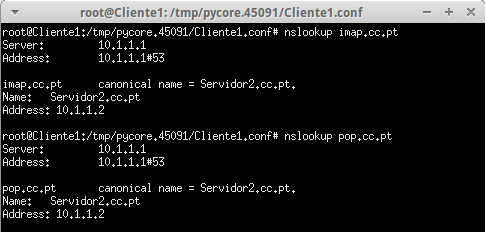
\includegraphics[scale=0.75]{teste9.png}
\end{center}
\caption{\label{fig:t9}Teste às funcionalidades do Servidor2}
\end{figure}

\begin{figure}[H]
\begin{center}
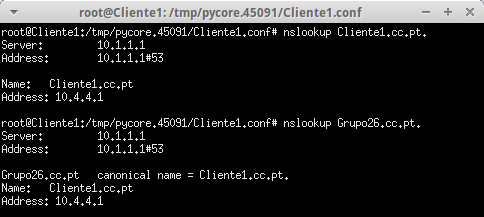
\includegraphics[scale=0.75]{teste10.png}
\end{center}
\caption{\label{fig:t10}Teste ao Cliente1}
\end{figure}

\begin{figure}[H]
\begin{center}
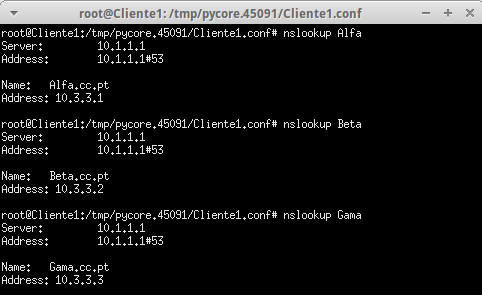
\includegraphics[scale=0.75]{teste11.png}
\end{center}
\caption{\label{fig:t11}Teste aos Hosts da zona 3}
\end{figure}



\end{document}
